\documentclass[12pt]{report}
\usepackage{scribe,graphicx,graphics}
\usepackage{amsmath}


\course{MIT 9.520/6.860} 	
\coursetitle{Statistical Learning Theory and Applications}	
\semester{Fall 2020}
%%% TODO: Fill in Lecturer's Name
\lecturer{Alice}
%%% TODO: Fill in the Lecture Title
\lecturetitle{What is Machine Learning?}
%%% TODO: Fill in Lecture Number
\lecturenumber{1}
%%% TODO: Fill in Lecture Date
\lecturedate{Oct 15th 1582}


%%%% TODO: Insert your name here!
\scribe{Bob, Charlie}

\begin{document}


\maketitle
\tableofcontents


\section{Introduction}
Fill in your Lecture Notes here. We have provided some basic \LaTeX formatting and commands in case you are unfamiliar; please remove them in the final document. 

\subsection{This is a subsection.}
Subsection text

\subsubsection{This is a sub-subsection}
Subsubsection text


\section{Some basic \LaTeX commands}

This is how you \emph{italicize} text; this is how to \textbf{bold} it. 

\subsection{Here's an equation:}
\begin{align}
    x = \frac{1}{2} = \left( \frac{2}{4} \right) = (0.5)
\end{align}

\subsection{Here's a boxed equation: }
\begin{align}
    \boxed{x = 1}
\end{align}

\subsection{Here's a list: }
\begin{enumerate}
    \item Here is an item in a list.
    \item Here's another item in a list.
\end{enumerate}

\subsection{Here's a figure:}

\begin{figure}[h]
    \centering
    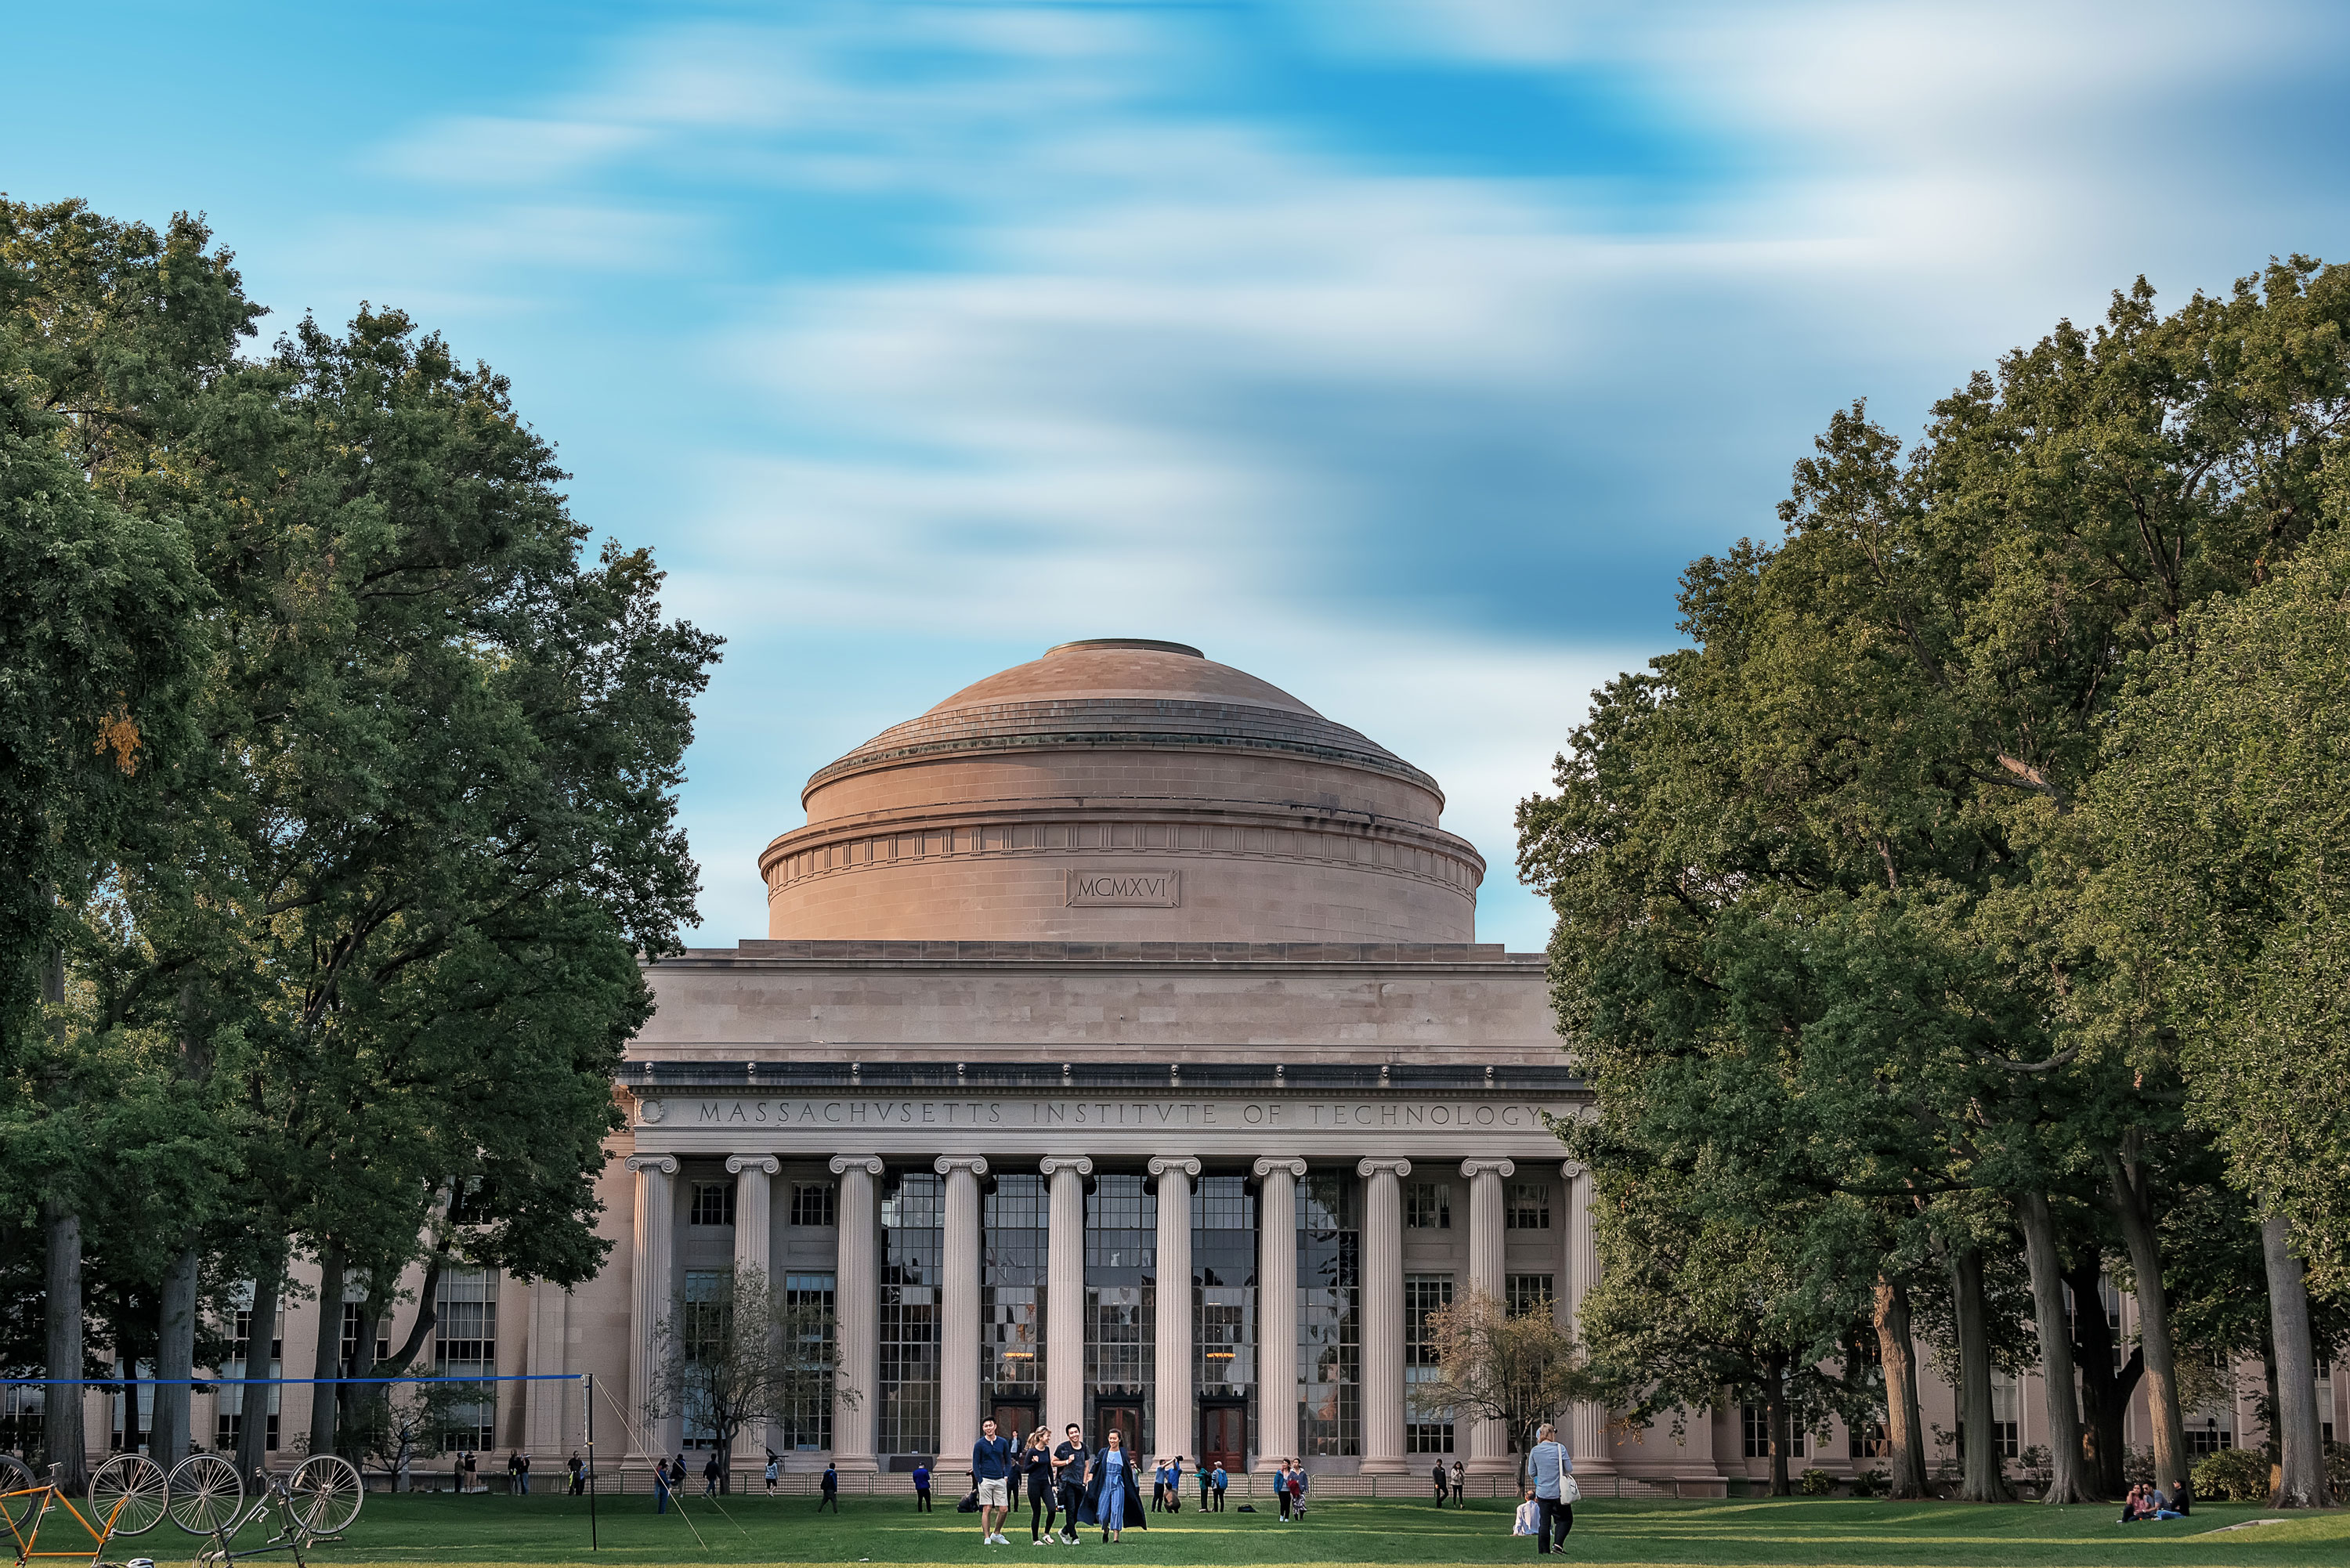
\includegraphics[width=0.5\textwidth]{topper_8-8.jpg}
    \caption{Caption}
    \label{fig:my_label}
\end{figure}


\end{document}

